\documentclass{beamer}
\mode<presentation>
% \usetheme{default}
% \usetheme{Boadilla}
% \usetheme{Madrid}
% \usetheme{Montpellier}
 \usetheme{Warsaw}
% \usetheme{Copenhagen}
% \usetheme{Goettingen}
% \usetheme{Hannover}
% \usetheme{Berkeley}
 
% \usecolortheme{crane}
 % \beamertemplatesolidbackgroundcolor{craneorange!25}
 
 \usepackage[utf8]{inputenc}
%\usepackage[T1]{fontenc}
\usepackage{amsmath,amssymb}
\usepackage[english,french]{babel}
%\usepackage{natbib}


 
\header{
\includegraphics[height=1.5cm]{phelma.jpg} \hfill 
\includegraphics[height=1.6cm]{cea.jpg} \hfill 
\includegraphics[height=1.6cm]{ujf.jpg}}
 

\title[Translocation de biomolécules à travers un nanopore]{Etude théorique de la translocation de biomolécules à travers un nanopore}




 
\author{Timothée Menais}
 
\institute[CEA] {
\includegraphics[height=1.4cm]{spram.jpg} \hspace{0.3cm}

\includegraphics[height=1.2cm]{inac.jpg}}


\setbeamertemplate{navigation symbols}{}


\begin{document}
\selectlanguage{french}

\frame[plain]{\titlepage} % # 1

\frame % 1
{
  \frametitle{Introduction}
 
 
 \begin{itemize}
 
 \begin{center}
 \item<1-> Translocation d'ADN à travers un nanopore
 
 \medskip
 \item<2-> Intérêts technologiques et fondamentaux
 
 \medskip
 \item<3> Arrivée du graphène
 \end{center}
 
 \end{itemize}


}





\section[Outline]{}
\frame{\tableofcontents}

\section{Outils analytiques}
 
 
\frame % # 2
{
  \frametitle{Statique}
 \begin{columns}
 \begin{column}{0.4\textwidth}

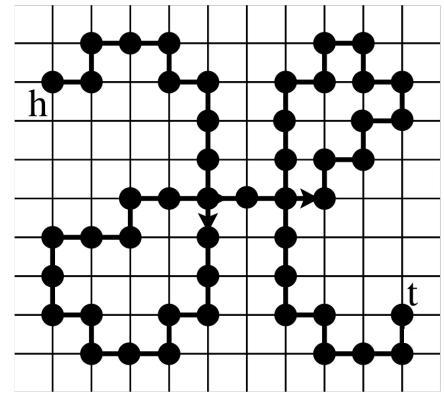
\includegraphics[width=\textwidth]{resideal.jpg}
\end{column}
\begin{column}{0.6\textwidth}



\begin{itemize}

\item<2->$Z_{ideal}=z^N \rightarrow Z_{non ideal} = \tilde{z}^N N^{\gamma-1}$ 
\medskip


 \item<3->$<\textbf{r}>=0$ et $<\textbf{r}^2>=d^2 t$
 \medskip

 
 \item<4->$R_0=\lambda N^{\frac{1}{2}} \rightarrow R_0=\lambda N^{\nu}$
 \medskip
 
 \item<5->$F(r) = F(0) + \frac{3 K_B T \textbf{r}^2}{2 R_0^2}$ de type ressort
\end{itemize}




 
\end{column}

\end{columns}


\vfill
{\tiny

\usebibitemtemplate{\color{structure}\insertbiblabel} 
\usebibliographyblocktemplate{\color{structure}}{\color{black}}{\color{structure!75}}{\color{structure!75}} 


\begin{thebibliography}{} 

\bibitem[référence]{these}
H Vocks. 
\newblock {Simulation of polymer translocation}. 
\newblock  Utrecht University, 2008. 

\end{thebibliography} }
}

 \frame % # 2
{
  \frametitle{Modèle de Rouse}
\centering
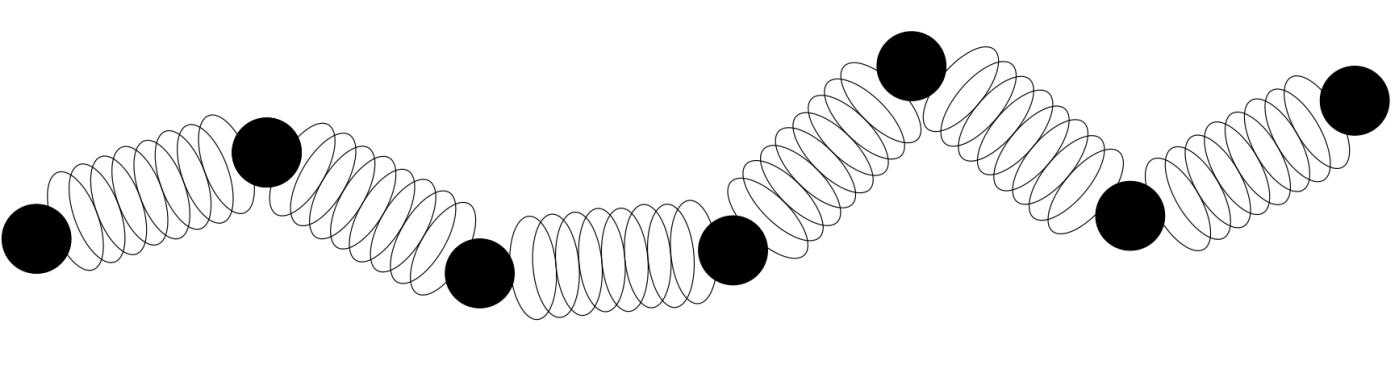
\includegraphics[width=0.8\textwidth]{rouse.jpg}






\begin{itemize}

\item<2-> \centering $\frac{d \textbf{r}_n}{dt} = -\frac{1}{\epsilon}\frac{\partial F_{tot}}{\partial \textbf{r}_n} +\textbf{g}_n$


\medskip

\item<3-> \begin{center} $<(\textbf{r}_{CM}(t)-\textbf{r}_{CM}(0))^2>=\frac{6 K_B T}{N \epsilon} t = 6 D_R t$\end{center}
\end{itemize}



\vfill
{\tiny

\usebibitemtemplate{\color{structure}\insertbiblabel} 
\usebibliographyblocktemplate{\color{structure}}{\color{black}}{\color{structure!75}}{\color{structure!75}} 

\begin{thebibliography}{} 
\bibitem[référence]{these}
H Vocks. 
\newblock {Simulation of polymer translocation}. 
\newblock Phd Thesis, Utrecht University, 2008. 

\end{thebibliography} }
}


}



 
\frame % 3
{
  \frametitle{Translocation}
 

\begin{columns}
 \begin{column}{0.8\textwidth}
\begin{center}
  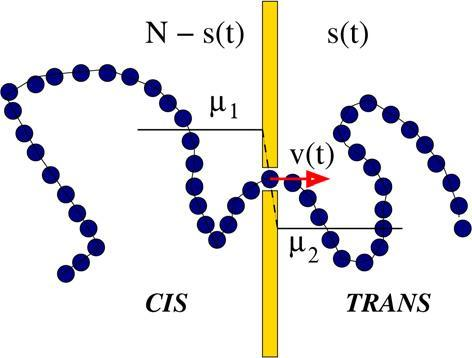
\includegraphics[width=0.8\textwidth]{translocation.jpg} 
 \end{center}
\end{column}
\begin{column}{0.2\textwidth}

 \begin{center}
\begin{itemize}
\item<2->{ $\tau = N^\alpha f^{-\delta}$}
\end{itemize}


\end{center}
 
\end{column}
\end{columns}

\vfill
{\tiny

\usebibitemtemplate{\color{structure}\insertbiblabel} 
\usebibliographyblocktemplate{\color{structure}}{\color{black}}{\color{structure!75}}{\color{structure!75}} 

\begin{thebibliography}{} 
\bibitem[référence]{milchev}
A Milchev. 
\newblock {Single-polymer dynamics under constraints: scaling theory and computer experiment}. 
\newblock J Phys Condens Matter 23(10):103101 (2011). 

\end{thebibliography} }
}



\frame % 3
{
  \frametitle{Translocation}
  
  \begin{center}
   $F(N,n) = K_B T [(1-\gamma_1)ln[n(N-n)] - Nln(\tilde{z})]$ 
   
    
   \medskip
   \uncover<2->{ $\tau$ est proportionnel à $\frac{R_0^2}{D}$ $_\tilde{}$ $N^{1+2\nu}$}
  \end{center}
 
 \uncover<3->{
 \begin{columns}
 \begin{column}{0.5\textwidth}
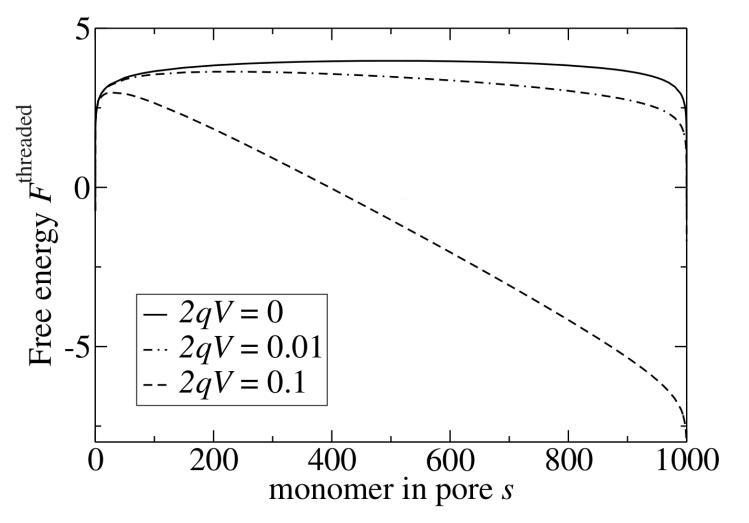
\includegraphics[width=\textwidth]{transelec.jpg}
\end{column}
\begin{column}{0.5\textwidth}

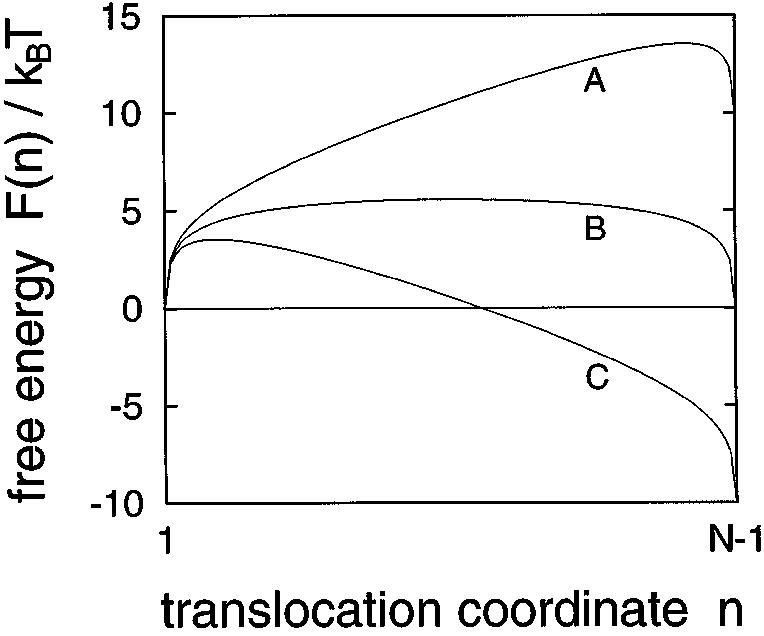
\includegraphics[width=0.9\textwidth]{transpotchim.jpg}
 
\end{column}
\end{columns}


}

\vfill
{\tiny

\usebibitemtemplate{\color{structure}\insertbiblabel} 
\usebibliographyblocktemplate{\color{structure}}{\color{black}}{\color{structure!75}}{\color{structure!75}} 

\begin{thebibliography}{} 
\bibitem[référence gauche]{these}
H Vocks. 
\newblock {Simulation of polymer translocation}. 
\newblock Phd Thesis, Utrecht University, 2008.

\bibitem[référence droite]{sung}
W. Sung and P. J. Park
k. 
\newblock {Polymer translocation through a pore in a membrane
}. 
\newblock Phys. Rev. Lett.,
vol. 77, pp. 783–786, Jul 1996. 

\end{thebibliography} }
}
}

\section{Dynamique moléculaire}

 \frame % # 2
{
  \frametitle{Nature de l'ADN}
  
  \begin{columns}
  \begin{column}{0.7\textwidth}
\begin{center}
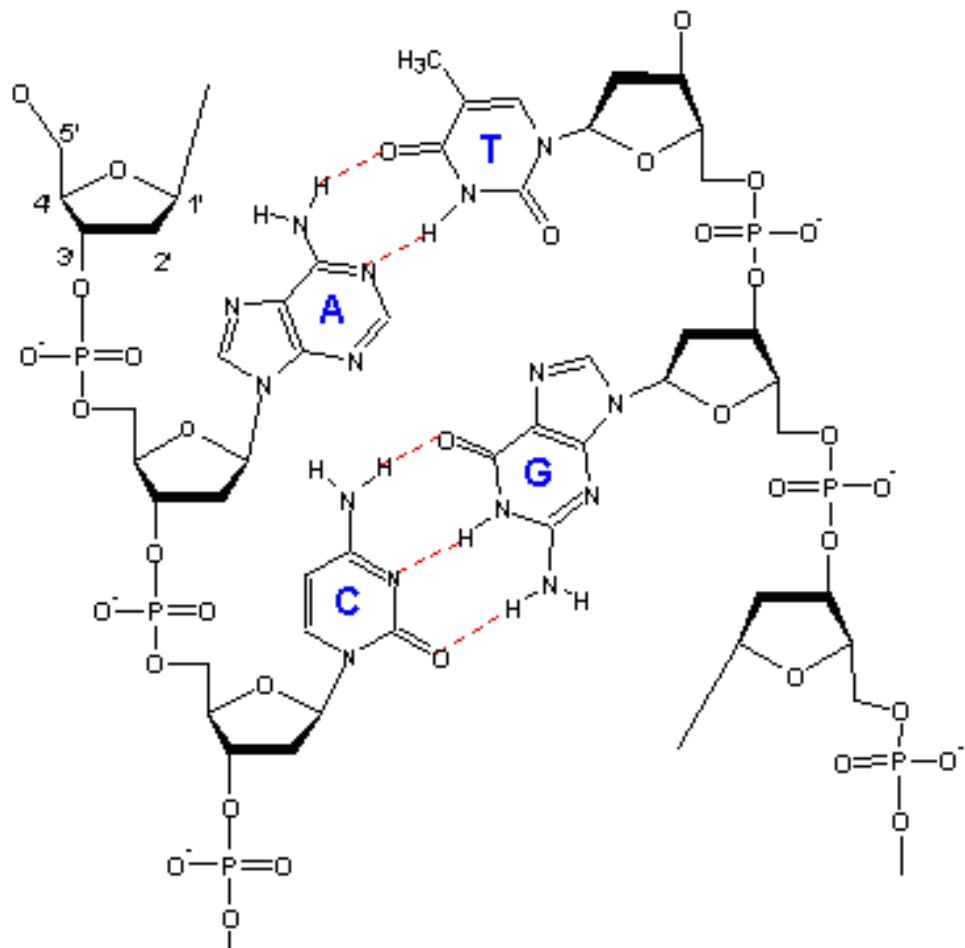
\includegraphics[width=0.8\textwidth]{adn.jpg}
\end{center}
\end{column}

  \begin{column}{0.3\textwidth}
\begin{center}
Structure\\
\medskip

Liaisons covalentes\\
\medskip

Liaisons hydrogènes\\
\medskip
Interactions orbitalaires


\end{center}
\end{column}

\end{columns}

}
\frame
{
  \frametitle{Modélisation}
  
\begin{center}
\hspace{3cm}

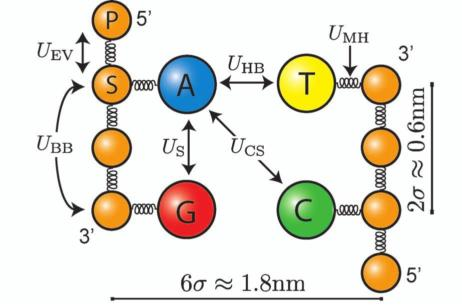
\includegraphics[width=0.6\textwidth]{moldyn2.jpg}
\end{center}
\begin{itemize}
\item<2-> \begin{center} $\frac{d \textbf{r}_n}{dt} = -\frac{1}{\epsilon}\frac{\partial F_{tot}}{\partial \textbf{r}_n} +\textbf{g}_n$\end{center}
\end{itemize}


\vfill
{\tiny

\usebibitemtemplate{\color{structure}\insertbiblabel} 
\usebibliographyblocktemplate{\color{structure}}{\color{black}}{\color{structure!75}}{\color{structure!75}} 

\begin{thebibliography}{} 
\bibitem[référence]{jchem}
M. C. Linak, R. Tourdot, and K. D. Dorfman. 
\newblock {Moving beyond watson–crick models of coarse grained
dna dynamics
}. 
\newblock The Journal of Chemical Physics, vol. 135, no. 20, p. 205102, 2011.
 

\end{thebibliography} }
}

}

\section{Graphène}

\frame % 3
{
  \frametitle{Graphène}

\begin{columns}
 \begin{column}{0.65\textwidth}
\begin{center}
  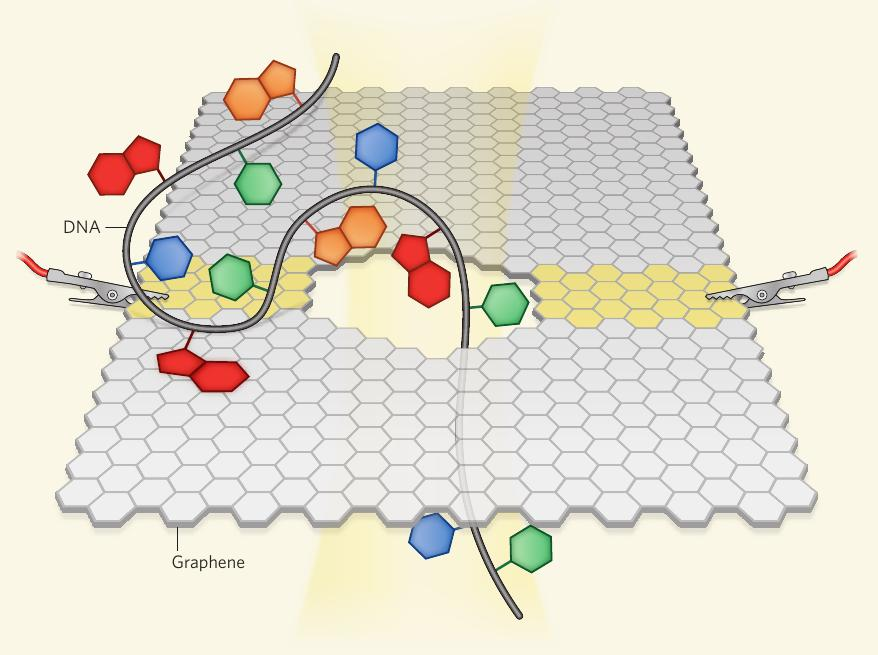
\includegraphics[width=\textwidth]{courant.jpg} 
 \end{center}
\end{column}
\begin{column}{0.35\textwidth}


 \begin{center}

anciens pores rigides:

biologiques et artificiels

\uncover<2->{
 
 
 problèmes d'épaisseur
}
\end{center}
 
\end{column}
\end{columns}

\vfill
{\tiny

\usebibitemtemplate{\color{structure}\insertbiblabel} 
\usebibliographyblocktemplate{\color{structure}}{\color{black}}{\color{structure!75}}{\color{structure!75}} 

\begin{thebibliography}{} 
\bibitem[référence]{graphen}
H. Bayley. 
\newblock {Nanotechnology : Holes with an edge
}. 
\newblock NATURE, vol. 467, p. 542,
SEP 2010. 

\end{thebibliography} }
}
}

}

\frame % 3
{
  \frametitle{Graphène}
 \begin{center}
  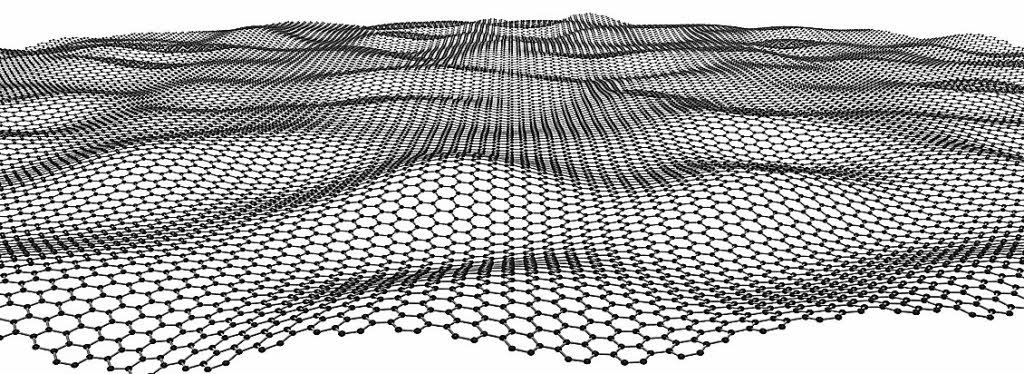
\includegraphics[width=0.8\textwidth]{vib.jpg} 
 \end{center}


}


\section*{Conclusion}

\frame % 3
{
  \frametitle{Conclusion}
 
 
 \begin{itemize}
 
 \begin{center}
 \item Utilisation d'outils analytiques et numériques
 \pause
 \medskip
 \item Modélisation du graphène
 \pause
 \medskip
 \item Temps de translocation, flexibilité et séquençage.
 \end{center}
 
 \end{itemize}


}

\frame % 3
{
  \frametitle{Conclusion}
 
 
 
 
 \begin{center}
 {\HUGE Merci de votre attention.
 
 
 \pause
 \medskip
 Des questions ?}
 \end{center}
 
 


}





\end{document}
       
 